\section{Introduction}

In the realm of data science and machine learning, the efficiency and effectiveness of data processing are often contingent upon the size and manageability of the datasets in use. The burgeoning volume of data necessitates innovative methods for reducing dataset size without compromising the integrity and utility of the data. This chapter focuses on validation tests for a revolutionary data size reduction method, applied to four well-known datasets: the Iris dataset, the Wine dataset, the Breast Cancer dataset, and the MNIST dataset.



\section{Tests done}
\subsection{Iris Dataset}

The Iris dataset, introduced by Ronald A. Fisher in 1936, is a staple in the field of machine learning and statistics. It consists of 150 instances of iris flowers, each described by four features: sepal length, sepal width, petal length, and petal width. These features are used to classify the flowers into three species: Iris-setosa, Iris-versicolor, and Iris-virginica. 

The simplicity and clarity of the Iris dataset make it an ideal candidate for demonstrating basic principles of data size reduction.

\begin{minipage}{0.6\textwidth}
    \centering
    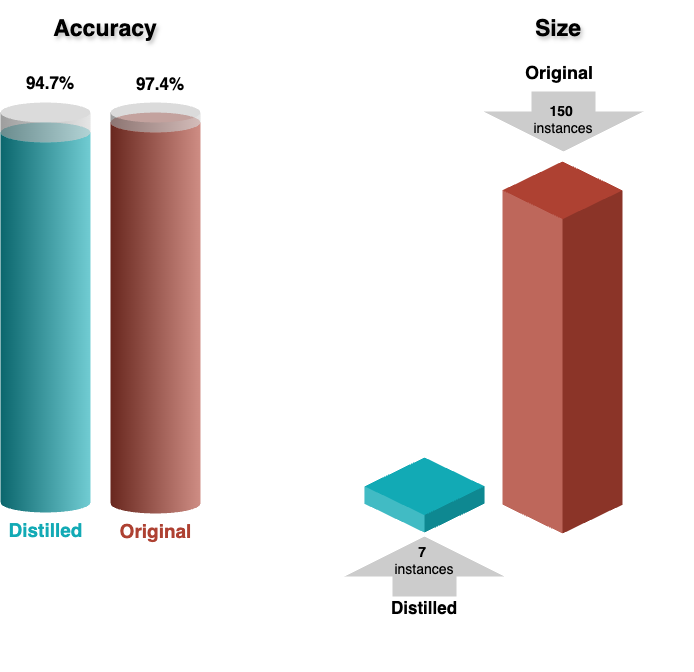
\includegraphics[width=\textwidth]{images/iris.png}
\end{minipage}
\hspace{0.02\textwidth} % Adjust this value to reduce the space
\begin{minipage}{0.35\textwidth}
    The figure illustrates the accuracy of a classifier trained on the original dataset, which contains 150 instances, achieving 97.4\% accuracy. In comparison, a model trained on a reduced dataset of 7 instances achieves 94.7\% accuracy. 
    
    This indicates that the proposed solution successfully reduces the original dataset by 95\% while maintaining a high classification accuracy of 94.7\%.
\end{minipage}

\subsection{Wine Dataset}

The Wine dataset is derived from the results of a chemical analysis of wines grown in the same region in Italy but derived from three different cultivars. It contains 178 instances with 13 attributes including alcohol content, malic acid, ash, and others. 

This dataset is often used for classification problems and serves as an excellent test bed for validating data reduction techniques due to its moderate size and complexity.

\begin{minipage}{0.35\textwidth}
    The figure shows the accuracy of a classifier trained on the original dataset of 178 instances, which achieves 97.8\% accuracy. In comparison, a model trained on a reduced dataset of 25 instances achieves 95.6\% accuracy. 
    
    This demonstrates that the proposed solution effectively reduces the original dataset by 86\% while maintaining a high classification accuracy of 95.6\%.
\end{minipage}
\hspace{0.02\textwidth} % Adjust this value to reduce the space
\begin{minipage}{0.6\textwidth}
    \centering
    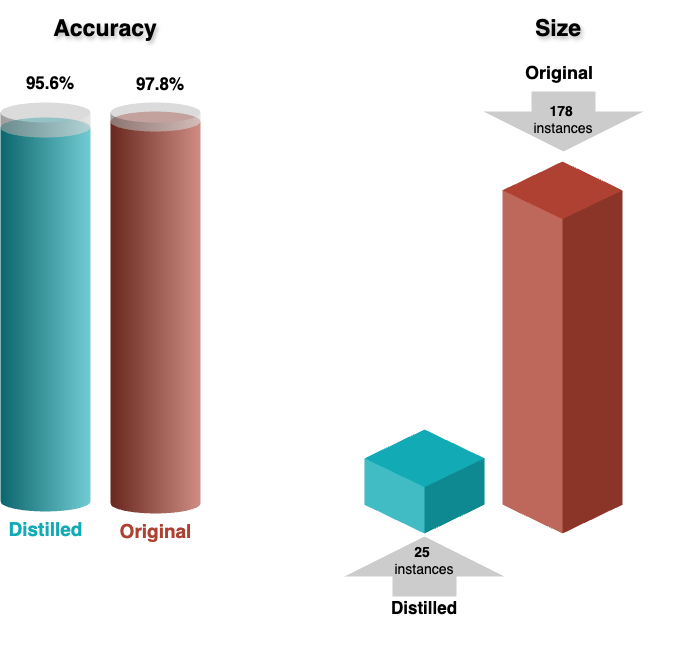
\includegraphics[width=\textwidth]{images/wine.png}
\end{minipage}


\subsection{Breast Cancer Dataset}

The Breast Cancer Wisconsin dataset, created by Dr. William H. Wolberg, is used for binary classification tasks in predicting the malignancy of breast cancer samples. It comprises 569 instances, each with 30 numeric features representing characteristics of cell nuclei present in a digitalized image of a fine needle aspirate of a breast mass. 

This dataset is critically important for medical research and diagnostics, making the preservation of data quality essential during size reduction.

\begin{minipage}{0.6\textwidth}
    \centering
    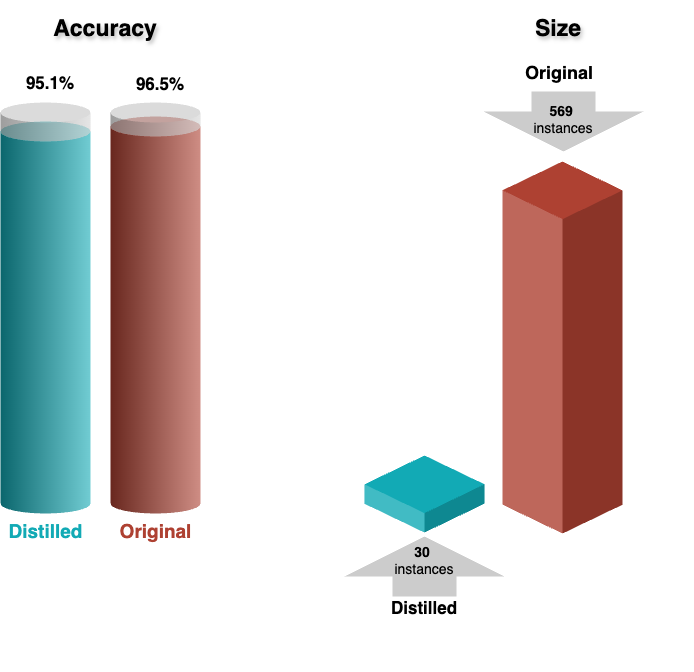
\includegraphics[width=\textwidth]{images/breast.png}
\end{minipage}
\hspace{0.02\textwidth} % Adjust this value to reduce the space
\begin{minipage}{0.35\textwidth}
The figure displays the accuracy of a classifier trained on the original dataset of 569 instances, which achieves 96.5\% accuracy. In comparison, a model trained on a reduced dataset of 31 instances achieves 95.1\% accuracy. 

This proofs that the proposed solution effectively reduces the original dataset by 95\% while maintaining a high classification accuracy of 95.1\%.
\end{minipage}


\subsection{MNIST Dataset}

The MNIST dataset is a large collection of handwritten digits, commonly used for training various image processing systems. It includes 60,000 training examples and 10,000 testing examples, each represented by a 28x28 grayscale image of a digit (0-9). 

The high dimensionality and substantial size of the MNIST dataset present significant challenges for data size reduction, thus providing a rigorous test for our proposed method.

\begin{minipage}{0.35\textwidth}
The figure shows the accuracy of a classifier trained on the original dataset of 70,000 instances, achieving 97.7\% accuracy. In comparison, a model trained on a reduced dataset of 4,424 instances achieves 93.7\% accuracy. 

This demonstrates that the proposed solution effectively reduces the original dataset by 93\% while maintaining a high classification accuracy of 93.7\%.
\end{minipage}
\hspace{0.02\textwidth} % Adjust this value to reduce the space
\begin{minipage}{0.6\textwidth}
    \centering
    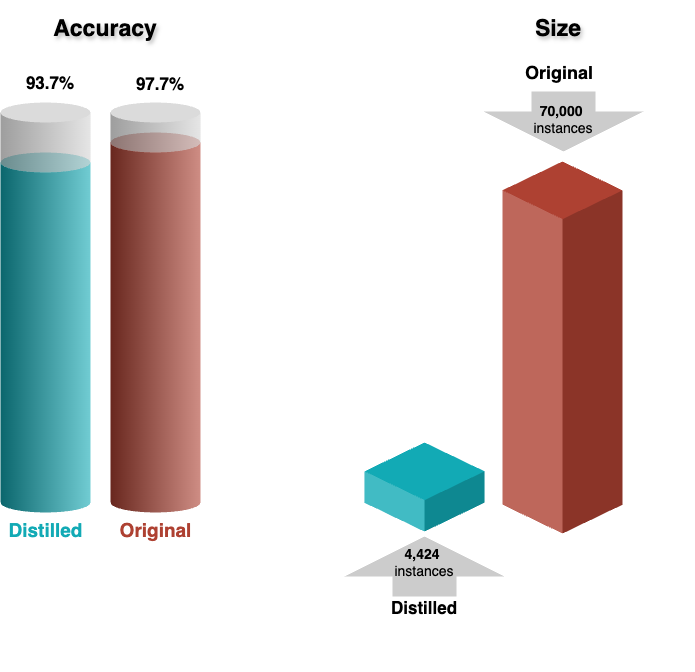
\includegraphics[width=\textwidth]{images/mnist.png}
\end{minipage}